\section{Results}
\label{sec:results}

Unless stated otherwise, local results cover the 1{,}200 prompts of the three
gradable families, costs are dynamic GPU energy in joules, and intervals are
95\% bootstrap intervals over prompts. Router results are on the test split
alone. The open-ended family, which carries the caveat of
Section~\ref{sec:setup-judge}, is reported separately in
Section~\ref{sec:results-open}.

\subsection{Oracle labels on the local grid}
\label{sec:results-labels}

Every gradable prompt was run through all eight cells: 9{,}600 generations in
386 measurement windows and 31.6 hours of GPU time. Twenty-six windows were
discarded under the rules of Section~\ref{sec:energy} and rerun, and no
accepted window was flagged as contaminated.

\begin{table*}[ht]
\centering
\small
\caption{The eight cells over the 1{,}200 gradable prompts, one sample per
prompt and cell. Accuracy counts a capped generation as a failure, and Capped
is the share of generations that reached the token cap. Tokens are input plus
output, reasoning included. Latency and energy are means per generation;
energy is dynamic board energy, and J per solved divides it by accuracy.}
\label{tab:cells}
\begin{tabular}{@{}lllrrrrrr@{}}
\toprule
Cell & Size & Mode & Acc.\ (\%) & Capped (\%) & Tokens & Latency (s) & Energy (J) & J per solved \\
\midrule
$c_1$ & 0.6B & no-think & 40.2 & 1.2 & 338 & 0.75 & 53.7 & 133.6 \\
$c_2$ & 0.6B & think & 53.0 & 18.9 & 1{,}862 & 6.53 & 490.9 & 926.2 \\
$c_3$ & 1.7B & no-think & 59.5 & 1.1 & 388 & 1.72 & 146.6 & 246.3 \\
$c_4$ & 1.7B & think & 65.0 & 19.9 & 2{,}107 & 13.85 & 1{,}022.8 & 1{,}573.5 \\
$c_5$ & 4B & no-think & 79.0 & 1.6 & 360 & 3.26 & 264.4 & 334.7 \\
$c_6$ & 4B & think & 76.8 & 16.2 & 1{,}904 & 25.35 & 1{,}837.0 & 2{,}393.5 \\
$c_7$ & 8B & no-think & 83.6 & 1.1 & 341 & 4.95 & 361.8 & 432.9 \\
$c_8$ & 8B & think & 79.8 & 16.5 & 1{,}980 & 42.57 & 2{,}880.3 & 3{,}611.7 \\
\bottomrule
\end{tabular}

\end{table*}

Table~\ref{tab:cells} gives the cells. Without thinking, accuracy rises at
every size step, from 40.2\% at 0.6B to 83.6\% at 8B, and energy per
generation from 54\,J to 362\,J. Thinking multiplies the output by 7.4 to 8.4
times and the energy by seven to nine. What that buys depends on size: it
adds 12.8 points at 0.6B and 5.5 at 1.7B, but loses 2.2 points at 4B and 3.8
at 8B. The loss sits in mathematics and tracks the cap: between 16\% and 20\%
of thinking generations reach 4{,}096 tokens at every size, against under 2\%
of non-thinking ones, and a truncated answer fails. On multiple choice
thinking helps at every size; on code it helps up to 4B and is level at 8B.
As a result, under a 4{,}096-token thinking budget the costliest cell is not
the most accurate one: $c_7$ answers 3.8 points more than $c_8$ for an eighth
of its energy. That ordering is a property of the configuration, budget
included, rather than of the model alone; Section~\ref{sec:results-mode}
reruns a sample of capped generations at 8{,}192 tokens and rescues a third
of them.

\begin{figure}[ht]
\centering
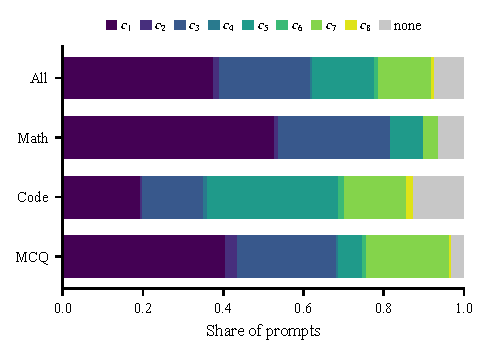
\includegraphics[width=\linewidth]{Figure_1}
\caption{The minimum sufficient cell $\cstar(q)$, in joules, over all prompts
and per family. ``None'' marks prompts that no cell answers.}
\label{fig:cstar}
\end{figure}

Fig.~\ref{fig:cstar} shows where the minimum sufficient cell falls. The
smallest model without thinking is $\cstar(q)$ for 37.5\% of prompts, and the
four non-thinking cells together for 89.2\%. A thinking cell is the cheapest
sufficient choice for 3.6\%, and $c_8$ for 0.75\%. No cell answers 7.25\% of
prompts: 12.5\% of code, 6.25\% of mathematics and 3.0\% of multiple choice.
The families differ in where the rest of the mass lies: on mathematics the
smallest cell suffices for 52.8\% of prompts, while on code the modal
$\cstar(q)$ is 4B without thinking, at 32.8\%.

Counted in tokens, the labels move up the grid. A non-thinking answer is
about as long at 8B as at 0.6B, 223 output tokens against 220, and the token
cost of \eqref{eq:tokcost} has no term for model size, so size is nearly free
and $\cstar(q)$ is $c_7$ for 31.3\% of prompts and $c_5$ for 26.9\%. In
energy an output token costs 0.24\,J at 0.6B and 1.6\,J at 8B. A token count
cannot see that factor of 6.6, and it drives several of the results below.
The attribution of energy within a window does not: apportioning each
window's dynamic energy by token share instead of generation time leaves
$\cstar(q)$ unchanged for 97.3\% of prompts, and per-generation energies
under the two rules have a rank correlation of 0.997.

\subsection{The escalation tax on the local grid}
\label{sec:results-tax}

\begin{table*}[ht]
\centering
\small
\caption{Escalation policies on the local grid over the 1{,}200 gradable
prompts, in joules. Cost per solved divides a policy's mean energy per prompt
by its solved rate, as in \eqref{eq:persolved}. The tax and its two
components are means over servable prompts, and the last column divides the
tax by the mean cost of $\cstar(q)$, 190.6\,J. Imperfect detection is the
illustrative point $p_{\mathrm{acc}} = 0.15$, $p_{\mathrm{rej}} = 0.05$.}
\label{tab:tax}
\begin{tabular}{@{}llrrrrrr@{}}
\toprule
Policy & Detection & Solved (\%) & Cost per solved [95\% CI] & Tax [95\% CI] & Esc. & Stk. & Tax / $c^*$ cost \\
\midrule
P1, frugal climb & oracle & 92.2 & 945.7 [803.2, 1{,}094.5] & 169.4 [139.8, 202.2] & 119.9 & 49.5 & 0.89 \\
P2, think first & oracle & 87.1 & 2{,}970.7 [2{,}634.2, 3{,}326.9] & 1{,}651.7 [1{,}454.7, 1{,}852.6] & 933.3 & 718.4 & 8.66 \\
P3, sticky high & oracle & 79.8 & 3{,}611.7 [3{,}388.3, 3{,}850.8] & 2{,}470.6 [2{,}364.2, 2{,}579.1] & 0.0 & 2{,}470.6 & 12.96 \\
P4, uniform start & oracle & 89.5 & 1{,}763.6 [1{,}603.1, 1{,}930.3] & 915.1 [861.6, 970.9] & 237.8 & 677.3 & 4.80 \\
P4, start skewed to $c_8$ & oracle & 85.3 & 2{,}503.9 [2{,}332.3, 2{,}678.9] & 1{,}581.8 [1{,}511.0, 1{,}653.8] & 135.9 & 1{,}445.9 & 8.30 \\
Random, then $c_8$ & oracle & 84.2 & 2{,}500.8 [2{,}309.9, 2{,}699.4] & 1{,}555.3 [1{,}463.8, 1{,}647.8] & 196.1 & 1{,}359.2 & 8.16 \\
Oracle & oracle & 92.8 & 634.8 [533.2, 741.1] & 0.0 [0.0, 0.0] & 0.0 & 0.0 & 0.00 \\
\midrule
P1, frugal climb & imperfect & 79.9 & 711.5 [613.4, 814.1] & 94.0 [75.1, 113.6] & 93.7 & 0.3 & 0.49 \\
P2, think first & imperfect & 74.9 & 2{,}302.4 [2{,}050.3, 2{,}568.4] & 1{,}093.3 [974.8, 1{,}213.3] & 603.9 & 489.4 & 5.74 \\
P3, sticky high & imperfect & 79.8 & 3{,}611.7 [3{,}388.3, 3{,}850.8] & 2{,}470.6 [2{,}364.2, 2{,}579.1] & 0.0 & 2{,}470.6 & 12.96 \\
P4, uniform start & imperfect & 84.5 & 1{,}659.2 [1{,}524.1, 1{,}799.0] & 877.2 [830.6, 925.6] & 213.5 & 663.7 & 4.60 \\
P4, start skewed to $c_8$ & imperfect & 82.4 & 2{,}468.6 [2{,}308.7, 2{,}633.0] & 1{,}560.1 [1{,}490.7, 1{,}630.4] & 122.0 & 1{,}438.1 & 8.18 \\
Random, then $c_8$ & imperfect & 81.4 & 2{,}440.6 [2{,}262.2, 2{,}626.7] & 1{,}485.9 [1{,}403.3, 1{,}568.8] & 181.1 & 1{,}304.8 & 7.79 \\
\bottomrule
\end{tabular}

\end{table*}

\begin{figure}[ht]
\centering
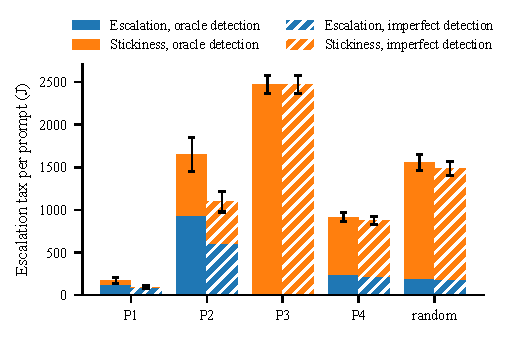
\includegraphics[width=\linewidth]{Figure_2}
\caption{The escalation tax per prompt, in joules, split into escalation and
stickiness, under oracle detection (solid) and imperfect detection (hatched).
Error bars are 95\% bootstrap intervals on the total. P4 starts uniformly
over the cells.}
\label{fig:tax}
\end{figure}

With every failure detected, each policy pays a tax whose interval excludes
zero (Table~\ref{tab:tax}, Fig.~\ref{fig:tax}). The oracle solves the 92.8\%
of prompts that some cell can answer, at 634.8\,J per solved prompt [533.2,
741.1].

Leaving the heaviest cell selected is the most expensive habit. P3 pays a tax
of 2{,}470.6\,J per prompt [2{,}364.2, 2{,}579.1], 12.96 times the cost of
$\cstar(q)$, and all of it is stickiness. It also solves the fewest prompts,
79.8\%, because $c_8$ is not the most accurate cell, and per solved prompt it
pays 3{,}611.7\,J, 5.7 times what the oracle pays. The frugal climb comes
close to the oracle: P1 solves 92.2\% of prompts at 945.7\,J per solved
prompt [803.2, 1{,}094.5], 1.5 times the oracle's figure, and its tax,
169.4\,J [139.8, 202.2] or 0.89 times the cost of $\cstar(q)$, is 71\%
escalation. Its first four rungs are the four cheapest cells, and between
them they are $\cstar(q)$ for 89.2\% of prompts, so the climb meets the
minimum sufficient cell in roughly the order an oracle would rank the cells.
Turning thinking on before moving up a size undoes this: P2 pays 8.66 times
and solves 87.1\%. The population policies fall between the extremes. P4 with
a uniform start pays 4.80 times, three-quarters of it stickiness; with half
of all queries starting at $c_8$ it pays 8.30 times, and random assignment
with recovery at $c_8$ pays 8.16 times. In every family P1 pays the least and
P3 the most.

Detection errors lower the tax and take answers with it. At the illustrative
point, P1's cost per solved prompt falls to 711.5\,J, because a wrong answer
accepted early ends the climb before the expensive rungs, and its solved rate
falls to 79.9\%, below both variants of P4. Every rung is another chance to
accept a wrong answer, so the policies that make the most attempts lose the
most: P1 loses 12.3 points and P2 12.2, while P4 with a uniform start loses
5.0. With no right answers rejected, P1's solved rate falls to P3's once one
wrong answer in five is accepted, 80.2\% against 79.8\%, though it still
spends 680\,J per solved prompt against P3's 3{,}612\,J. Oracle detection is
therefore the regime in which the manual policies answer the most prompts,
not the one in which they spend the least.

The unit changes the ranking. Measured in tokens, P3's tax falls to 4.40
times the cost of $\cstar(q)$ while P2's stays at 8.65, and per solved prompt
P3 spends 2{,}482 tokens against P2's 4{,}719. Tokens charge P2 for every
thinking rung and charge P3 almost nothing for model size, so a token count
ranks sticking with the largest model as the cheaper of the two habits.
Measured energy ranks it as the more expensive, 3{,}611.7\,J per solved
prompt against 2{,}970.7\,J.

\subsection{Routing on the local grid}
\label{sec:results-routing}

\begin{table*}[ht]
\centering
\scriptsize
\caption{Routers on the 243 test prompts, in joules, with a failed routed
answer recovered at $c_8$ and every failure detected. Net cost is the mean
energy per prompt with the router's own energy included; its interval is for
the first training seed, and the standard deviation across three seeds
follows in parentheses. Saving and the change in solved rate are paired
differences against P1, positive when the router is cheaper or solves more,
with Holm-corrected $p$-values. Area is the normalised area under the
router's cost--quality frontier as $\tau$ varies. For the cascade, $\tau$ is
its verification threshold.}
\label{tab:routers}
\setlength{\tabcolsep}{4pt}
\begin{tabular}{@{}lrrrrrrr@{}}
\toprule
Policy or router & $\tau$ & Solved (\%) & Net cost [95\% CI] (s.d.) & Saving vs.\ P1 [95\% CI] & $\Delta$ solved (pp) & $p_{\mathrm{Holm}}$ & Area \\
\midrule
Always $c_8$ & -- & 81.1 & 2{,}676.8 [2{,}430.2, 2{,}926.7] & -- & -- & -- & -- \\
P1, frugal climb & -- & 92.2 & 831.5 [578.2, 1{,}122.1] & -- & -- & -- & -- \\
Random, then $c_8$ & -- & 84.7 & 1{,}896.5 [1{,}633.7, 2{,}170.2] & -- & -- & -- & -- \\
Oracle & -- & 93.0 & 565.5 [377.3, 775.3] & -- & -- & -- & -- \\
\midrule
Direct: TF-IDF + LR & -- & 85.6 & 1{,}521.3 [1{,}249.4, 1{,}803.1] (0.0) & -689.8 [-909.3, -478.8] & -6.6 [-9.9, -3.7] & 0.009 & 0.377 \\
TF-IDF + LR & 0.84 & 88.5 & 1{,}041.0 [801.0, 1{,}304.7] (0.0) & -209.5 [-363.6, -67.7] & -3.7 [-6.2, -1.6] & 0.029 & 0.551 \\
TF-IDF + LR (cost-sens.) & 0.66 & 86.4 & 1{,}162.7 [894.6, 1{,}450.2] (0.0) & -331.2 [-512.7, -164.2] & -5.8 [-8.6, -2.9] & 0.009 & 0.549 \\
Features + LightGBM & 0.76 & 87.7 & 1{,}213.5 [960.1, 1{,}480.7] (102.5) & -382.0 [-562.2, -209.8] & -4.5 [-7.4, -2.1] & 0.009 & 0.479 \\
Features + LightGBM (cost-sens.) & 0.84 & 86.8 & 1{,}209.7 [940.6, 1{,}500.6] (71.2) & -378.2 [-580.8, -191.2] & -5.3 [-8.2, -2.9] & 0.009 & 0.499 \\
Features + XGBoost & 0.84 & 86.8 & 1{,}318.7 [1{,}058.2, 1{,}599.0] (84.1) & -487.2 [-671.6, -315.2] & -5.3 [-8.2, -2.9] & 0.009 & 0.477 \\
Features + XGBoost (cost-sens.) & 0.80 & 87.7 & 1{,}185.2 [919.8, 1{,}469.1] (15.0) & -353.7 [-550.5, -170.3] & -4.5 [-7.4, -2.1] & 0.009 & 0.517 \\
MiniLM + LR & 0.74 & 86.8 & 1{,}156.1 [894.5, 1{,}436.9] (0.0) & -324.6 [-504.6, -161.0] & -5.3 [-8.2, -2.9] & 0.009 & 0.553 \\
MiniLM + LR (cost-sens.) & 0.72 & 87.7 & 1{,}069.8 [821.6, 1{,}339.4] (0.1) & -238.3 [-404.0, -88.9] & -4.5 [-7.4, -2.1] & 0.025 & 0.539 \\
DeBERTa-v3-small & 0.94 & 86.4 & 1{,}491.7 [1{,}218.1, 1{,}786.2] (40.8) & -660.2 [-875.6, -450.8] & -5.8 [-8.6, -2.9] & 0.009 & 0.389 \\
DeBERTa-v3-small (cost-sens.) & 1.00 & 86.4 & 1{,}216.2 [950.5, 1{,}500.9] (128.5) & -384.7 [-567.2, -212.9] & -5.8 [-9.1, -2.9] & 0.009 & 0.433 \\
DistilBERT & 0.92 & 85.6 & 1{,}649.7 [1{,}349.3, 1{,}964.9] (48.4) & -818.2 [-1{,}055.0, -596.6] & -6.6 [-9.9, -3.7] & 0.009 & 0.382 \\
DistilBERT (cost-sens.) & 0.90 & 86.4 & 1{,}130.6 [876.2, 1{,}408.5] (9.7) & -299.1 [-468.5, -143.7] & -5.8 [-9.1, -2.9] & 0.009 & 0.518 \\
Qwen3-0.6B, few-shot & 0.86 & 83.5 & 1{,}872.9 [1{,}583.8, 2{,}168.2] (0.0) & -1{,}041.4 [-1{,}287.8, -797.7] & -8.6 [-12.3, -5.3] & 0.009 & 0.262 \\
Qwen3-0.6B, LoRA & 0.80 & 86.4 & 1{,}262.9 [994.2, 1{,}540.6] (46.8) & -431.4 [-622.1, -248.6] & -5.8 [-9.1, -2.9] & 0.009 & 0.466 \\
Qwen3-0.6B, zero-shot & 0.16 & 84.8 & 1{,}594.6 [1{,}307.2, 1{,}891.4] (0.0) & -763.1 [-998.1, -530.7] & -7.4 [-11.1, -4.1] & 0.009 & 0.366 \\
AutoMix-style cascade & 0.98 & 85.6 & 1{,}587.2 [1{,}305.4, 1{,}880.2] (--) & -755.8 [-971.6, -549.6] & -6.6 [-9.9, -3.7] & 0.009 & 0.355 \\
\bottomrule
\end{tabular}

\end{table*}

\begin{figure}[ht]
\centering
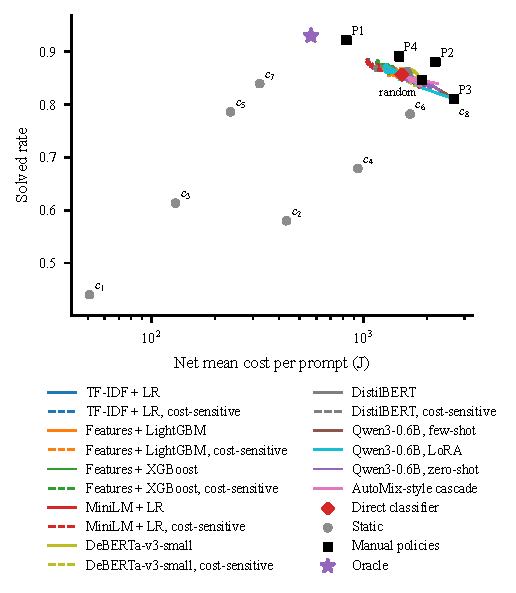
\includegraphics[width=\linewidth]{Figure_3}
\caption{Solved rate against net mean energy per prompt on the test split:
each router as $\tau$ varies (dashed for cost-sensitive training), the
cascade as its threshold varies, the eight cells used alone, the manual
policies and the oracle. Cost is logarithmic.}
\label{fig:frontier}
\end{figure}

Routers were trained on 716 prompts, had $\tau$ chosen on 241 and were
evaluated once on the remaining 243, on which P1 solves 92.2\% at 831.5\,J
per prompt [578.2, 1{,}122.1] and the oracle 93.0\% at 565.5\,J.

Under this recovery rule no router beats the frugal climb, and neither does
the cascade (Table~\ref{tab:routers}); the rule matters, and we return to it
below. The best router,
logistic regression on TF-IDF $n$-grams, solves 88.5\% at 1{,}041.0\,J
[801.0, 1{,}304.7], which is 209.5\,J more than P1 [67.7, 363.6] and 3.7
points fewer [1.6, 6.2]; its net energy per solved prompt is 1.30 times P1's
[1.10, 1.63]. Every other router and the cascade also spends more than P1 and
solves fewer prompts, with Holm-corrected $p \leq 0.03$ in every case. The
shortfall belongs to the routers, not the grid: the oracle spends 32\% less
than P1 [24, 41].

Against the habits that start high, the same router removes most of the tax.
Charged for its own energy, it spends 61\% less than P3 [53, 69] and solves
7.4 points more [4.1, 10.7]; 52\% less than P2 [43, 60]; 45\% less than
random assignment [37, 53]; and 29\% less than P4 with a uniform start [23,
36] at a solved rate within a point of it.

The loss to P1 sits in recovery. A routed answer that fails is resent to
$c_8$, the costliest cell and a less accurate one than $c_7$. The TF-IDF
router guards against that with a high threshold, $\tau = 0.84$: of the test
prompts some cell can answer, it sends 76.1\% to a costlier cell than
$\cstar(q)$ that still succeeds, 9.7\% to a cell that fails and 14.2\%
exactly to $\cstar(q)$, so its tax, 2.70 times the cost of $\cstar(q)$, is
95\% stickiness where P1's is mostly escalation. When a failed routed answer
instead climbs the P1 ladder from the routed cell, the gap closes: every
router then lies within 6\% of P1's energy per solved prompt, solving the
same share of prompts or at most 1.2 points fewer, and four are 2.6\% to
3.4\% cheaper than P1 (Holm-corrected $p = 0.009$).

Imperfect detection reverses the comparison of solved rates. At the
illustrative point P1 solves 80.3\% of prompts, because each of its 1.92
attempts is another chance to accept a wrong answer, while the TF-IDF router
makes 1.18 attempts and solves 87.4\%, which is 7.1 points more [4.2, 9.7],
at 1.76 times P1's energy per solved prompt [1.50, 2.16].

The cascade loses to most routers. It solves 85.6\% at 1{,}587.2\,J per
prompt, and 11 of the 15 one-shot routers are significantly cheaper, the
TF-IDF router by 34\% [23, 45] ($p = 0.002$). Its verification checks are not
the reason, at 9.7\,J each: the check a model runs on its own answer accepts
a wrong one on 33.6\% of the prompts some cell can answer, and each of those
goes to $c_8$ as a misrouted one does, so the cascade makes 2.39 attempts per
prompt, more than any router.

Charging each router for its own energy changes little. No router costs more
than 7.6\,J per decision, 0.6\% of the energy of the queries it routes, and
only three routers change rank between gross and net cost, all within 7\,J of
one another. In tokens the charge matters: the R3 routers pay for their own
prompts, 281 tokens per decision zero-shot and 1{,}141 few-shot, and the LoRA
router falls from fifth to eleventh of 17. The verdict against P1 also
depends on the unit. The TF-IDF router needs 1.35 times P1's latency per
solved prompt [1.13, 1.69] but only 0.76 times its tokens [0.65, 0.89],
because in tokens a failed small attempt costs about as much as an answer
from $c_7$, so P1's climb is dear, while in energy it is nearly free.

Ranked by their best member, the router families keep their order gross and
net. Logistic regression on TF-IDF $n$-grams and on frozen MiniLM embeddings
rank first and second. The fine-tuned encoders approach them only with
cost-sensitive training, which lowered DistilBERT's net cost from
1{,}649.7\,J to 1{,}130.6\,J; it did not help the TF-IDF router. The prompted
R3 routers finish last, beside the cascade: asked for the cheapest sufficient
configuration, the 0.6B model routes low, and the few-shot prompt sends
52.7\% of answerable prompts to a cell that fails. Predicting success per
cell also beats classifying $\cstar(q)$ directly, by 480.3\,J per prompt with
the same TF-IDF features [241.6, 723.8]. The linear routers give the same
result with every training seed, while the gradient-boosted and fine-tuned
ones vary with standard deviations of up to 128.5\,J. Table S4 of the
supplementary material gives each router's overhead per decision.

\subsection{Energy of the reasoning-mode axis}
\label{sec:results-mode}

\begin{figure}[ht]
\centering
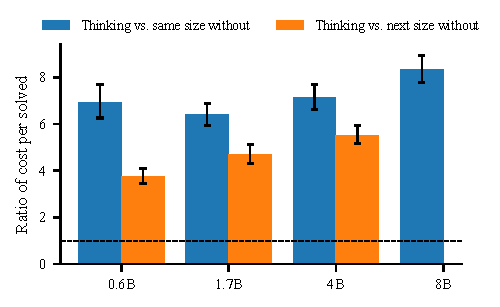
\includegraphics[width=\linewidth]{Figure_4}
\caption{Energy per solved prompt with thinking, relative to the same size
without thinking and to the next size up without thinking. Error bars are
95\% bootstrap intervals, and the dashed line marks parity. 8B has no next
size.}
\label{fig:mode}
\end{figure}

Thinking does not cost a fixed multiple of non-thinking energy
(Fig.~\ref{fig:mode}). Per solved prompt it costs 6.9 times as much as the
same model without thinking at 0.6B, 6.4 times at 1.7B, 7.2 at 4B and 8.3 at
8B, and the intervals at 1.7B, [5.9, 6.9], and 8B, [7.8, 8.9], do not
overlap. The ratio varies more by family than by size: on mathematics it
stays between 4.9 and 6.1, on code it reaches 12.9 at 4B and 15.8 at 8B, and
on multiple choice it peaks at 0.6B, at 15.2, where a non-thinking answer
costs 10\,J.

Under these budgets thinking is also never the cheaper way to buy accuracy on
this grid. Below 8B, the next size up without thinking answers more prompts
than thinking does---59.5\% against 53.0\% at 0.6B, 79.0\% against 65.0\% at
1.7B and 83.6\% against 76.8\% at 4B---and spends 3.8, 4.7 and 5.5 times less
energy per solved prompt, with intervals of [3.5, 4.1], [4.3, 5.1] and [5.1,
6.0]. The same holds in every family, with two exceptions in accuracy: on
code at 0.6B thinking answers 2.8 points more than 1.7B without it, at 4.5
times the energy per solved prompt, and on multiple choice at 4B the two tie.

This conclusion does not wait for the cap reruns. Suppose every capped
thinking generation had been correct, at the energy it used before it was cut
off; thinking would then answer 71.9\%, 84.9\% and 93.0\% of prompts at 0.6B,
1.7B and 4B, more than the next size up at every step, and would still spend
2.8, 3.6 and 4.6 times as much energy per solved prompt. The bound favours
thinking twice over, since an answer that needs a longer budget also needs
more energy. The reruns confirm it: of 219 capped generations rerun with an
8{,}192-token budget, 32.4\% succeed and 27.9\% reach the longer cap as well.
The share rescued rises with size for thinking, from 15.0\% at 0.6B to 52.5\%
at 8B, and the answers it buys are long: a rescued 8B thinking answer has a
median of 5{,}201 output tokens and 8.6\,kJ, against a mean of 362\,J for an
8B non-thinking generation. A rescue moves $\cstar(q)$ for 6.4\% of the rerun
generations and makes 4.6\% of them servable.

Within a size, the premium is one of length. A thinking generation spends
between 0.94 and 1.15 times the energy per output token of a non-thinking
generation at the same size, so output tokens price the mode axis to within
about 15\%, while they miss the factor of 6.6 between sizes.

\subsection{Asymmetry of misallocation}
\label{sec:results-asymmetry}

A router's two errors are priced by sending each servable prompt to the tier
just below its $\cstar(q)$ and to the tier just above, with a failed answer
recovered at $c_8$ as a router's would be. Tiers are the cells in order of
mean energy, $c_1, c_3, c_5, c_7, c_2, c_4, c_6, c_8$, so a step up in energy
is not always a step up in accuracy: the tier above $c_7$ is 0.6B with
thinking. One tier too low fails on 79.8\% of the 663 prompts that have a
lower tier and costs 2{,}625.9\,J more than $\cstar(q)$ [2{,}461.8,
2{,}790.1], 13.8 times its mean cost. One tier too high fails on 24.1\% of
the 1{,}104 prompts that have a higher tier and costs 968.6\,J more [861.4,
1{,}080.8]. Routing too low is therefore 2.71 times as costly [2.43, 3.04] in
energy and 2.85 times [2.55, 3.19] in latency, most on mathematics, at 3.44,
and least on multiple choice, at 1.91.

That is a factor of about three rather than ten, and in tokens the asymmetry
reverses, to 0.86 [0.77, 0.97]. The non-thinking cells lie within 50 tokens
of one another, so their token order has little to do with size: the tier
below $c_3$ is 4B and the tier below $c_5$ is 8B. A step down in tokens then
succeeds on 62\% of prompts, while a step up is often to a thinking cell
whose output is several times as long. In energy and latency, then, a router
should demand more confidence before it routes a prompt down than before it
routes it up, which a threshold $\tau$ above one half does and an argmax over
$\cstar(q)$ does not.

\subsection{Open-ended requests}
\label{sec:results-open}

The open-ended family is reported with the caveat fixed in advance. The local
judge reaches $\kappa = 0.42$ [0.23, 0.59] against the blind human scores,
inside the caveat band, and it is lenient: it passes 65\% of the human
sample, against 57\% for the human rater and 50\% for
\texttt{gpt-5-mini}. The success rates below are therefore those of a lenient
grader; leniency raises every cell's rate, and how it moves $\cstar(q)$
between cells is not known.

On these prompts the grid behaves differently from the gradable families.
Accuracy rises with size and with thinking at every step, from 46.3\% at
$c_1$ to 86.3\% at $c_8$, so here the costliest cell is also the most
accurate, and the cap barely binds: no cell has more than 1.25\% of its
generations reach it. Thinking costs 1.9 to 2.1 times the energy per solved
prompt of the same size without it, against 6.4 to 8.3 on the gradable
families, because a plain open-ended answer is already long and a
generation's tokens only about double with thinking. At 0.6B thinking is
cheaper than the next size up, at 0.62 times the energy per solved prompt of
1.7B without thinking [0.56, 0.71]. A thinking cell is therefore the cheapest
sufficient choice for 22.8\% of open-ended prompts, against 3.6\% of gradable
ones.

The ordering of the policies survives. P1 still pays the least, a tax of 1.46
times the cost of $\cstar(q)$ [1.14, 1.86], and solves 93.8\% of prompts; P3
pays 5.39 times [4.29, 6.85] and solves 86.3\%. The spread is narrower than
on the gradable families because $c_8$ costs 6.5 times the mean cost of
$\cstar(q)$ here rather than 14 times, and is also the most accurate cell. P2
comes close to P1, at 1.79 times, because its second rung, 0.6B with
thinking, is a cheap and useful step on this family. Routing one tier too low
costs 2.03 times as much as one tier too high [1.75, 2.38]. Over all four
families, 1{,}600 prompts, P3 pays 10.59 times the cost of $\cstar(q)$ and P1
1.07 times.

\subsection{The escalation tax on a public benchmark}
\label{sec:results-public}

\begin{table*}[ht]
\centering
\small
\caption{Escalation policies on the public pool under oracle detection, in US
dollars per 1{,}000 queries. P1 climbs the cost--accuracy frontier, P3 uses
its top rung once, P4 starts uniformly over the pool and then climbs, and
Random picks a model uniformly and recovers at the top rung. A policy that
answers fewer queries can show a negative tax, underpaying by failing, so the
tax is read beside the solved column.}
\label{tab:public}
\setlength{\tabcolsep}{4pt}
\begin{tabular}{@{}lrrrrr@{}}
\toprule
Policy & Solved (\%) & Attempts & Cost (\$/1{,}000) [95\% CI] & Tax [95\% CI] & Tax / $c^*$ cost \\
\midrule
P1, climb the frontier & 76.2 & 2.27 & 43.73 [41.98, 45.54] & 16.12 [15.11, 17.17] & 2.69 \\
P3, sticky top & 58.8 & 1.00 & 60.02 [58.62, 61.41] & 47.74 [46.41, 49.04] & 7.96 \\
P4, uniform start & 71.0 & 1.83 & 54.03 [52.34, 55.77] & 28.28 [27.25, 29.29] & 4.72 \\
Random, then top & 64.5 & 1.50 & 47.22 [45.82, 48.61] & 29.48 [28.44, 30.51] & 4.92 \\
\midrule
Always \texttt{deepseek-v3-0324} & 41.3 & 1.00 & 0.76 [0.74, 0.79] & -5.31 [-5.86, -4.78] & -0.89 \\
Always \texttt{qwen3-235b-a22b-2507} & 53.3 & 1.00 & 0.84 [0.81, 0.87] & -5.27 [-5.82, -4.75] & -0.88 \\
Always \texttt{gpt-5} & 57.6 & 1.00 & 29.15 [28.31, 30.01] & 18.34 [17.69, 19.01] & 3.06 \\
Always \texttt{gemini-2.5-pro} & 58.8 & 1.00 & 60.02 [58.62, 61.41] & 47.74 [46.41, 49.04] & 7.96 \\
\midrule
Oracle & 82.0 & 1.00 & 20.88 [19.84, 21.96] & 0.00 [0.00, 0.00] & 0.00 \\
\bottomrule
\end{tabular}

\end{table*}

The public pool spans a factor of 79 in price, from \$0.76 to \$60.02 per
thousand queries, and a factor of 1.6 in accuracy, from 36.9\% to 58.8\%.
Price and accuracy are only loosely related: of the eleven models dearer than
\texttt{qwen3-235b-a22b-2507}, nine answer fewer queries than it does. Only
four of the thirteen lie on the cost--accuracy frontier (Figure~S5 of the
supplementary material), and those four are the ladder a rational escalator
would climb; between them the thirteen answer 82.0\% of the queries. The
distribution of the minimum sufficient model repeats what the local grid
shows: the two cheapest models are the cheapest sufficient choice for 46.5\%
of queries and the costliest model for 2.4\%, while another 29.8\% are
answered most cheaply by a model off the frontier.

Table~\ref{tab:public} gives the policies. Sticky use of the top of the
ladder (P3) pays a tax of 7.96 times the minimum sufficient cost and answers
58.8\% of queries; climbing the frontier (P1) pays 2.69 times, answers 76.2\%
and takes 2.27 attempts per query; the oracle answers 82.0\% at \$20.88 per
thousand. Per solved query the ordering is the same and the comparison is
fair across policies of unequal success: \$25.47 for the oracle, \$57.38 for
P1 and \$102.08 for P3, so a user who always reaches for the strongest model
pays four times what a perfect one-shot router would pay for the same
answers.

Two features of the pool are worth separating from the local grid. First, the
frontier is a subset: a policy climbing it fails on queries only an
off-frontier model answers, and then pays four cheap attempts instead of one
expensive sufficient model. This is why the two cheapest static policies show
a negative tax, and why on SimpleQA even P1 does; they underpay by failing,
which is why cost per solved query carries the comparison. Second, the dollar
tax is larger than the token tax---7.96 against 2.04 for P3---because the
price per token spans two orders of magnitude across providers while the
answers themselves do not differ in length nearly as much. Escalation on a
mixed pool is expensive in a way token counts hide.

The thinking and non-thinking releases of Qwen3-235B-A22B give the public
counterpart of the mode axis. Thinking costs 9.11 times more per solved query
[8.78, 9.47] and, over all nine datasets, answers slightly fewer queries
(52.1\% against 53.3\%). Only 9.3\% of queries need it, so the mode is worth
paying for on a small minority and is picked per query or not at all. Where
reasoning is the point the picture reverses---on GPQA thinking answers 80.3\%
against 58.6\%---which is the same family-dependence the local grid shows.
Scoring a judged Arena-Hard tie as half credit rather than requiring a full
score moves nothing: P3 pays 8.14 times and P1 2.64 times, against 7.96 and
2.69.

\subsection{The escalation tax on a hosted frontier ladder}
\label{sec:results-hosted}

\begin{table*}[ht]
\centering
\small
\caption{Escalation policies on the hosted ladder under oracle detection, in
US dollars per 1{,}000 queries. The static rows are the ladder rungs used
alone. As on the public pool, a policy that answers fewer queries can show a
negative tax by underpaying through failure, so the tax is read beside the
solved column.}
\label{tab:hosted}
\setlength{\tabcolsep}{4pt}
\begin{tabular}{@{}lrrrrr@{}}
\toprule
Policy & Solved (\%) & Attempts & Cost (\$/1{,}000) [95\% CI] & Tax [95\% CI] & Tax / $c^*$ cost \\
\midrule
P1, climb the frontier & 97.1 & 1.38 & 0.34 [0.26, 0.44] & 0.04 [-0.01, 0.09] & 0.22 \\
P2, costly mode first & 97.2 & 1.38 & 0.86 [0.62, 1.14] & 0.26 [0.15, 0.39] & 1.41 \\
P3, sticky top & 92.8 & 1.00 & 1.02 [0.96, 1.09] & 0.80 [0.72, 0.87] & 4.35 \\
P4, uniform start & 95.1 & 1.15 & 1.57 [1.46, 1.69] & 1.27 [1.17, 1.36] & 6.93 \\
Random, then top & 94.6 & 1.12 & 1.61 [1.50, 1.73] & 1.33 [1.22, 1.43] & 7.24 \\
\midrule
Always $h_{1}$ & 74.2 & 1.00 & 0.03 [0.03, 0.03] & -0.15 [-0.23, -0.09] & -0.84 \\
Always $h_{3}$ & 89.5 & 1.00 & 0.18 [0.17, 0.19] & -0.01 [-0.08, 0.05] & -0.04 \\
Always $h_{5}$ & 91.8 & 1.00 & 0.79 [0.74, 0.85] & 0.59 [0.51, 0.65] & 3.20 \\
Always $h_{4}$ & 92.8 & 1.00 & 1.02 [0.96, 1.09] & 0.80 [0.72, 0.87] & 4.35 \\
\midrule
Oracle & 97.5 & 1.00 & 0.25 [0.18, 0.33] & 0.00 [0.00, 0.00] & 0.00 \\
\bottomrule
\end{tabular}

\end{table*}

The six hosted cells, over the 825 prompts every cell answered, span a factor
of 185 in price, from \$0.03 to \$5.77 per thousand queries, and 74.2\% to
92.8\% in accuracy. Four lie on the cost--accuracy frontier (Figure~S6) and form the ladder
$h_1 \rightarrow h_3 \rightarrow h_5 \rightarrow h_4$: \texttt{gpt-5-nano},
then \texttt{gpt-5-mini} at minimal effort, then \texttt{gpt-5} at minimal
effort, then \texttt{gpt-5-mini} at high effort. Both cells left off the
ladder are high-effort ones. \texttt{gpt-5-nano} at high effort costs twice
\texttt{gpt-5-mini} at minimal and answers twelve points fewer, and
\texttt{gpt-5} at high effort, the costliest cell at 5.6 times the price of
\texttt{gpt-5-mini} at high effort, answers slightly fewer queries than it,
91.9\% against 92.8\%. The most expensive thing a user can buy here is not
the most accurate one.

The cheapest cell is the minimum sufficient choice for 74.2\% of queries and
the second rung for another 16.0\%; 2.5\% are answered by no cell, and paid
reasoning effort is the cheapest sufficient choice for 5.1\% across its three
cells. Table~\ref{tab:hosted} gives the policies: P3 pays a tax of 4.35 times
the minimum sufficient cost and answers 92.8\%, P1 pays 0.22 times, answers
97.1\% and takes 1.38 attempts, and the oracle answers 97.5\% at \$0.25 per
thousand. Per solved query P3 pays \$1.10 against the oracle's \$0.25, so
escalation on this ladder is a factor of 4.4 on the price of an answer.
Starting uniformly over the six cells and then climbing (P4) pays 6.93 times,
more than either, because two of its six starting points are cells the
frontier excludes. One static policy is worth naming: \texttt{gpt-5-mini} at
minimal effort used alone costs within noise of the minimum sufficient
cost---a tax of $-0.04$ [$-0.32$, 0.41]---while answering 89.5\% of queries.

The reasoning-effort axis is priced here rather than metered, and the price
is a multiple rather than a margin: high effort costs 11.8, 5.45 and 7.26
times minimal effort at \texttt{gpt-5-nano}, \texttt{gpt-5-mini} and
\texttt{gpt-5}. What it buys shrinks as the model gets stronger. The share of
queries minimal effort fails and high effort answers is 15.2\% at
\texttt{gpt-5-nano}, 6.2\% at \texttt{gpt-5-mini} and 4.1\% at
\texttt{gpt-5}, where overall accuracy moves by a tenth of a point, from
91.8\% to 91.9\%, and falls on multiple choice from 94.9\% to 93.4\%.

The cap does to the hosted cells what it does to the local grid.
\texttt{gpt-5-nano} at high effort spends 1{,}845 reasoning tokens on the
average prompt and hits its 4{,}096-token cap on 18.9\% of them. Counting a
truncated generation as a failure leaves it at 77.8\%; on the responses that
finish it answers 96.0\%, against 74.5\% for the same model at minimal
effort. On code, where its reasoning runs longest, high effort is worse than
minimal outright, 65.3\% against 82.5\%. Reasoning that does not fit the
budget is paid for and discarded, which is the same failure the local 0.6B
and 1.7B thinking cells show.

Because the hosted prompts are the local main subset, each has a $\cstar(q)$
on both ladders, and 765 of the 825 are servable in both; the hosted cells
answer 39 of the 55 prompts the local pool cannot, 24 of them at its two
cheapest rungs, and 16 defeat both. What does not carry across is the rank:
on the prompts both arms answer, the correlation between how far up its own
ladder a prompt must be sent locally and on the hosted ladder is 0.05
($p = 0.16$), so a prompt that needs a large local model is not the one that
needs an expensive hosted tier. The mode axis carries better: the cheap mode
is the cheapest sufficient choice for 96.2\% of the locally servable prompts
and minimal effort for 96.1\% of the hosted ones, and both hold together for
92.8\%. A router trained on one pool therefore transfers its reasoning-mode
decision more readily than its size decision.

\subsection{Carbon of the escalation tax}
\label{sec:results-carbon}

Carbon is energy multiplied by a grid intensity, so a grid rescales every
policy by the same factor and cannot reorder them; what a bracket of
intensities shows is how the choice of policy compares with the choice of
grid. Per 1{,}000 queries, P3's tax is 34\,g of CO$_2$e on a grid at
50\,gCO$_2$e/kWh and 480\,g at 700; P1's is 2.4\,g and 33\,g. Leaving the
largest model selected on a low-carbon grid therefore emits about as much
excess carbon as the frugal climb on a coal-heavy one, the tax differing by a
factor of 14.6 between the two policies where the bracket spans a factor of
14. These are board-level figures for one laptop GPU, and Table S5 of the
supplementary material gives the full bracket.
